\section{Experimental Results}
\label{sec:4_5_Expsetup}

The objective of the experiments conducted in this study was to evaluate the efficacy of multiclass oversampling techniques in enhancing the performance of the first proposed method in imbalanced drifted multiclass classification streams. Our primary goal was to develop a novel approach that combines Dynamic Ensemble Selection (DES) to improve classification performance and robustness in such streams. These experiments yielded valuable insights that could further refine the performance of the first proposed approach and its ability to effectively handle imbalanced data streams. These findings provide a better understanding of the capabilities of the first proposed approach and offer insights into an optimal strategy for tackling minority class issues and concept drift in imbalanced data streams. This study contributes to the advancement of stream mining techniques for generating more accurate and robust classification models in dynamic data stream environments. By addressing the challenges posed by minority classes and concept drift, this study offers valuable insights for improving the performance of the first proposed approach and enhancing the overall efficiency of stream mining.

\subsection{Experimental setup}
The evaluation of the first proposed approach incorporated the utilization of various metrics such as recall, precision, specificity, $f_1$ score, balanced accuracy score (BAC), and geometric mean score (G-mean) \cite{bu2016pdf}. The experimental protocol utilized for evaluation was the test-then-train approach \cite{venkatasubramanianinformation}, where the classification classifier was trained on a specific data chunk and subsequently evaluated on the subsequent one. The chunk size was standardized for all utilized data streams to 2,000 instances. Four classification classifiers are employed as base estimators: K-Nearest Neighbor (KNN), Support Vector Machine (SVM), Gaussian Naive Bayes (GNB), and Hoeffding Tree (HT), as implemented in scikit-learn \cite{frias2014online}. A pool of classifiers was constructed with a maximum size of $L$ = 8, where the DES selected the best classifier for each chunk. If the pool surpassed the set threshold ($L$), the classifier with the lowest performance was eliminated. The experiments were conducted using Python programming language, and the source code was publicly available on GitHub\footnote{\url{https://github.com/Amadkour/dynamic__classification_ensembles_for_handling_imbalanced_multi-class_drifted_data_streams.git}} . A comparison was conducted between multiclass oversampling techniques (MLSMOTE and MLSOL) and the first proposed approach to demonstrate the effectiveness of the contribution. Additionally, these experiments are conducted that uses two different concept drift detectors, ADWIN \cite{storkey2008training} and DDM \cite{losing2016knn}, to demonstrate the adaptability and robustness of first proposed approach across varying drift detectors.

\subsection{Data Streams}
In this study, the first approach was assessed using various datasets including benchmark datasets, a real application stream dataset, and synthetic data streams. The Stream-learn Python library was used to conduct the evaluations \cite{dries2009adaptive}. Table \ref{tab:4_first_proposal_result_table_1} illustrates the benchmark dataset employed in this study, which consists of the Covertype dataset containing 40 features, seven classes, and 581,010 instances. For real application stream evaluation, the Sensor stream dataset was used, which consisted of five features, 58 classes, and 392,600 instances. This represents a real-world application scenario and provides valuable insights into the performance of the first proposed approach in practical settings. Synthetic datasets were generated using Scikit-learn Python library to evaluate the performance of the first proposed approach. The synthetic dataset was designed to simulate data streams and comprised 10 features and four classes divided into 200 chunks of 2,000 instances each. The performance of the first approach was systematically evaluated using these datasets and a stream-learn library. These evaluations provided insights into the effectiveness of the first approach in handling different types of data streams, including benchmark datasets, real application streams, and synthetic data streams.

\begin{table}[H]
  \centering
  \caption{Summary of Dataset Characteristics Utilized in the PA1 Experimental.}
  \resizebox{\textwidth}{!}{
  \begin{tabular}{|l|c|c|c|}
  \hline
  \textbf{Dataset} & \textbf{Number of Features} & \textbf{Number of Classes} & \textbf{Number of Instances} \\ \hline
  Covertype dataset\footnote{\url{http://archive.ics.uci.edu/dataset/31/covertype}} & 40 & 7 & 581,010 \\ \hline
  Sensor Stream dataset\footnote{\url{https://www.cse.fau.edu/~xqzhu/Stream/sensor.arff}} & 5 & 58 & 392,600 \\ \hline
  Synthetic stream & 8 & 3 & 200,000 \\ \hline
  \end{tabular}
  }
  \label{tab:4_first_proposal_result_table_1}
  \end{table}

\subsection{Analysis of Experimental Results}
The performance of the first proposed approach was comprehensively assessed on multiple data streams, considering two distinct concept drift detectors, ADWIN and DDM. To ensure thorough evaluation, six key performance metrics—$f_1$ score, recall, precision, G-mean, specificity, and balanced accuracy—were carefully presented using two visualization diagrams: radar and line. A radar diagram was strategically utilized to provide an overview that effectively depicted the performance of each algorithm across the six metrics. The mean value of each metric was calculated to present the overall performance of each method (MLSMOTE, MLSOL, PA1). It is important to note that the PA1 is represented by red lines.

\subsubsection{Results on the Benchmark Stream}

Figures \ref{fig:4_first_proposal_result_exp_1} and \ref{fig:4_first_proposal_result_exp_2} unveil the intricate dynamics of applying MLSMOTE, MLSOL, and PA1 to the Covertype dataset under the guidance of ADWIN and DDM as drift detectors. These figures not only explore the multifaceted nature of classifier ensemble adaptation but also illustrate the critical role of drift detection mechanisms in shaping performance metrics, including G-mean—a pivotal metric that encapsulates the delicate balance between sensitivity (recall) and specificity.
\vspace{-3mm}
\begin{figure}[H]
	\centering
	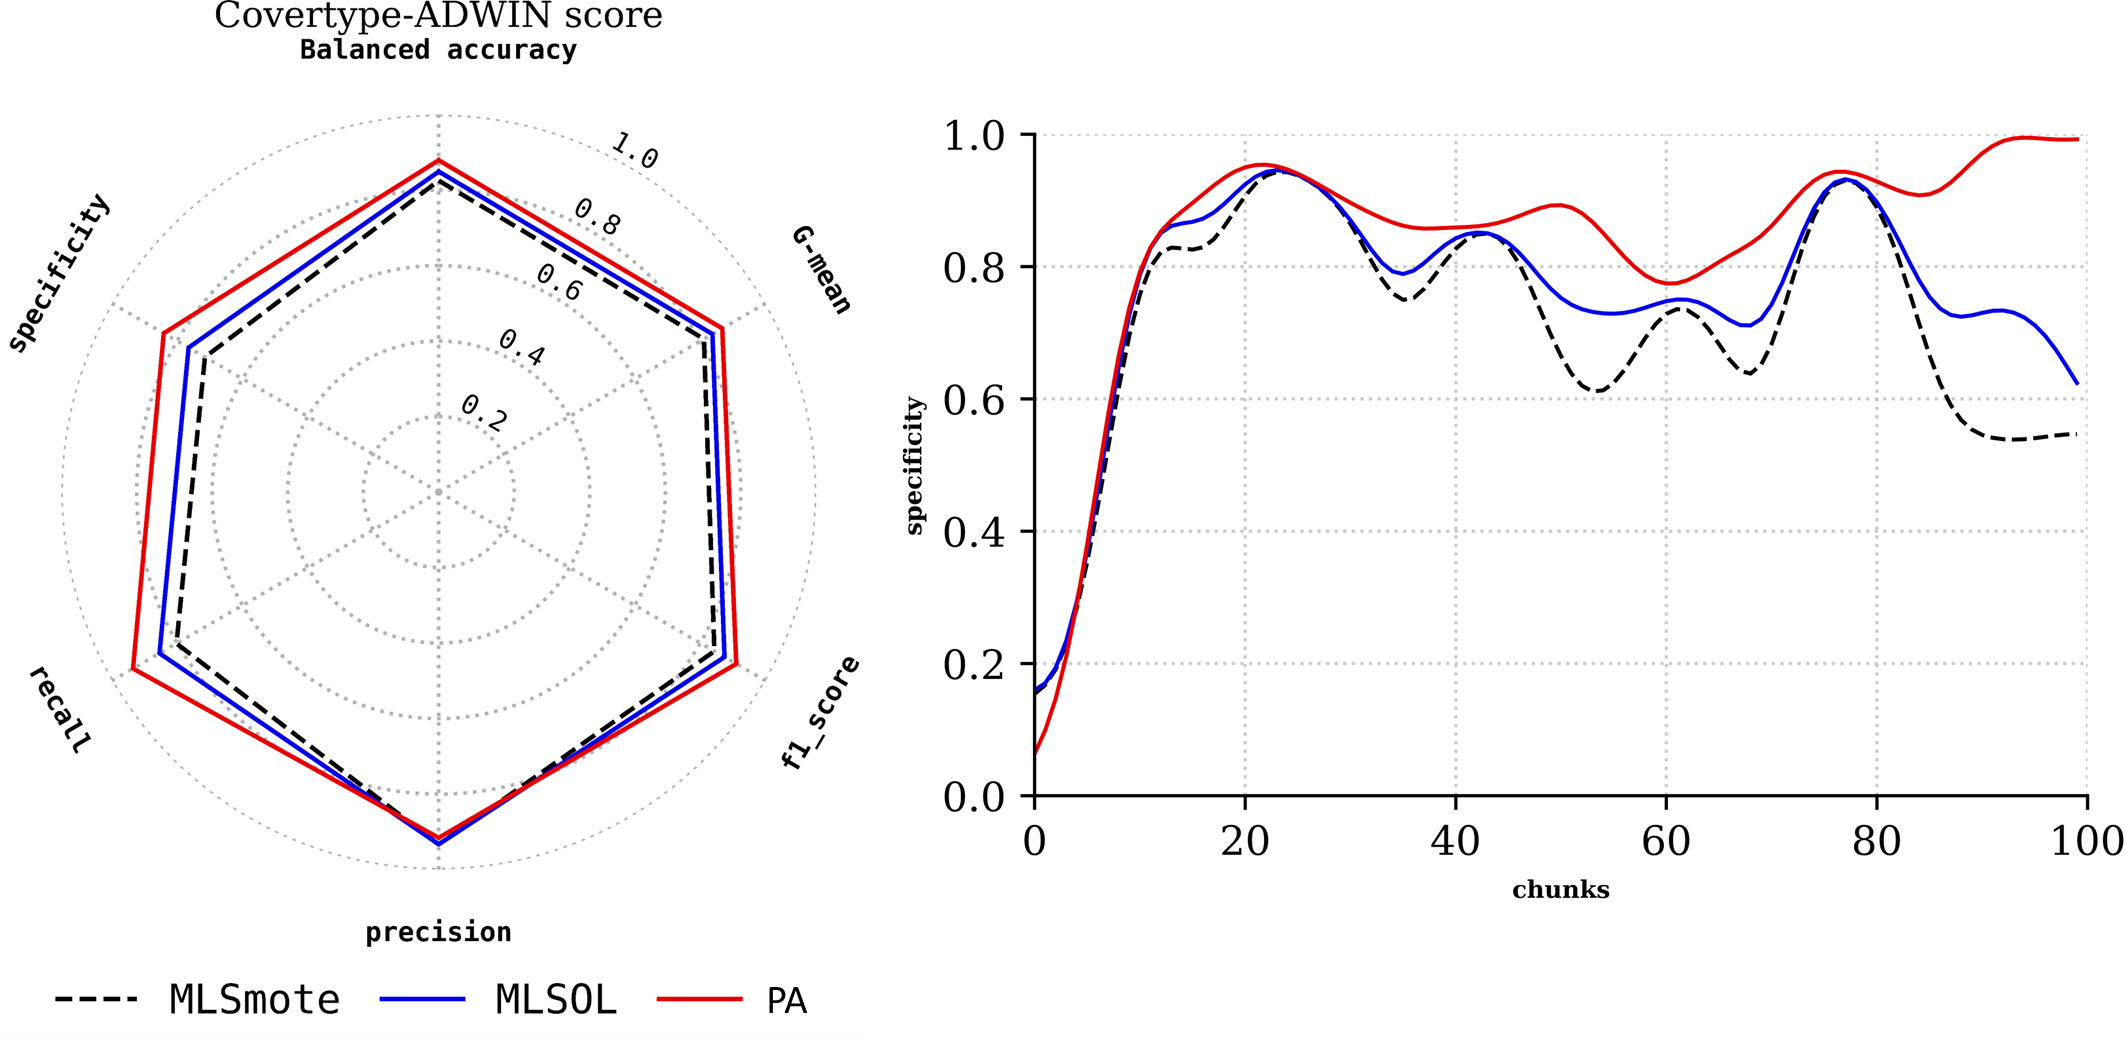
\includegraphics[width=1\linewidth]{4_Imbalanced/figures/exp_1.png}
	\caption{Comparison of PA1, MLSMOTE, and MLSOL on Covertype Dataset with ADWIN Concept Drift Detector.}
	\label{fig:4_first_proposal_result_exp_1}
\end{figure}
In Figure \ref{fig:4_first_proposal_result_exp_1}, ADWIN’s influence is evident as the radar diagram vividly portrays the comparative performance of the three methods across six critical metrics: precision, recall, specificity, $f_1$ score, G-mean, and balanced accuracy. PA1, symbolized by the red line, asserts its dominance by consistently outperforming MLSOL (blue line) and MLSMOTE (dashed black line). Its superior performance in G-mean reflects a methodical synergy between precision and recall, highlighting PA1’s ability to reconcile conflicting objectives in stream classification. In contrast, MLSOL offers a more conservative, balanced performance, excelling marginally in specificity but faltering in achieving broader metric optimization. MLSMOTE, by comparison, reveals fundamental limitations, as its deficiencies in recall and balanced accuracy suggest a struggle to maintain consistent adaptability and robustness in evolving data streams. The temporal evolution of classification performance, captured in the line diagram, provides deeper insights into the relationship between the chunk number and specificity values. During the first 20 chunks, all three methods exhibit suboptimal specificity scores, a reflection of the inherent challenges posed by the initialization phase, where the classifier pool is still adapting to the data distribution. However, as the number of chunks increases, PA1 demonstrates a marked improvement in specificity, particularly between chunks 20 and 40, where its strategic use of historical knowledge allows it to dynamically optimize its classifier ensemble. This ability to leverage past chunks for generating non-overlapping, representative samples underscores PA1’s resilience, enabling it to maintain a consistently high specificity throughout subsequent chunks. In contrast, MLSOL exhibits moderate growth in specificity, benefiting from its localized learning strategies but lagging behind PA1 due to its less aggressive approach to historical knowledge utilization. MLSMOTE, however, consistently trails its counterparts, as its limited adaptability and inability to reconcile recall and specificity prevent it from achieving competitive specificity values. The gradual stabilization of specificityvalues beyond chunk 40 for PA1 and MLSOL indicates the maturation of their classifier pools, while the relative stagnation of MLSMOTE underscores its inefficacy in addressing long-term concept drift.
Figure \ref{fig:4_first_proposal_result_exp_2}, which incorporates DDM as the drift detector, provides a complementary perspective. The radar plot mirrors the performance hierarchy observed with ADWIN, albeit with a slight degradation in metric values across all methods. This decline reflects DDM’s inherent limitations in capturing subtle shifts in data distribution, resulting in less precise ensemble adaptations. The line diagram further reinforces this observation, as specificityvalues exhibit reduced stability compared to ADWIN. While PA1 retains its dominance, the performance gap between PA1, MLSOL, and MLSMOTE narrows, suggesting that the rigidity of DDM diminishes the relative advantage conferred by PA1’s historical knowledge strategies. The interplay between chunk number and specificity in Figure \ref{fig:4_first_proposal_result_exp_2} reveals a similar trend: all methods struggle in the early stages due to limited classifier diversity, but PA1’s strategic design enables it to recover more effectively than its counterparts. Despite this, the overall reduction in specificity values highlights DDM’s comparative inefficiency in adapting to concept drift, particularly in scenarios characterized by rapid and unpredictable changes.
These figures underscore the profound influence of drift detection mechanisms on classifier ensemble performance. ADWIN’s demonstrated superiority in fostering stable and adaptive specificity trajectories highlights the importance of dynamic, context-sensitive drift detection in navigating the complexities of evolving data streams. Meanwhile, PA1’s sustained excellence exemplifies the philosophical alignment of algorithmic design with the realities of non-stationary environments. Its ability to harmonize sensitivity and specificity, as evidenced by consistently high specificity values across chunks, marks it as a paradigm for robust and adaptive learning in machine learning research. By contrast, the limitations of MLSMOTE and MLSOL serve as reminders of the challenges inherent in balancing local adaptation with global coherence in dynamic, heterogeneous data environments.

\vspace{-2mm}
\begin{figure}[H]
	\centering
	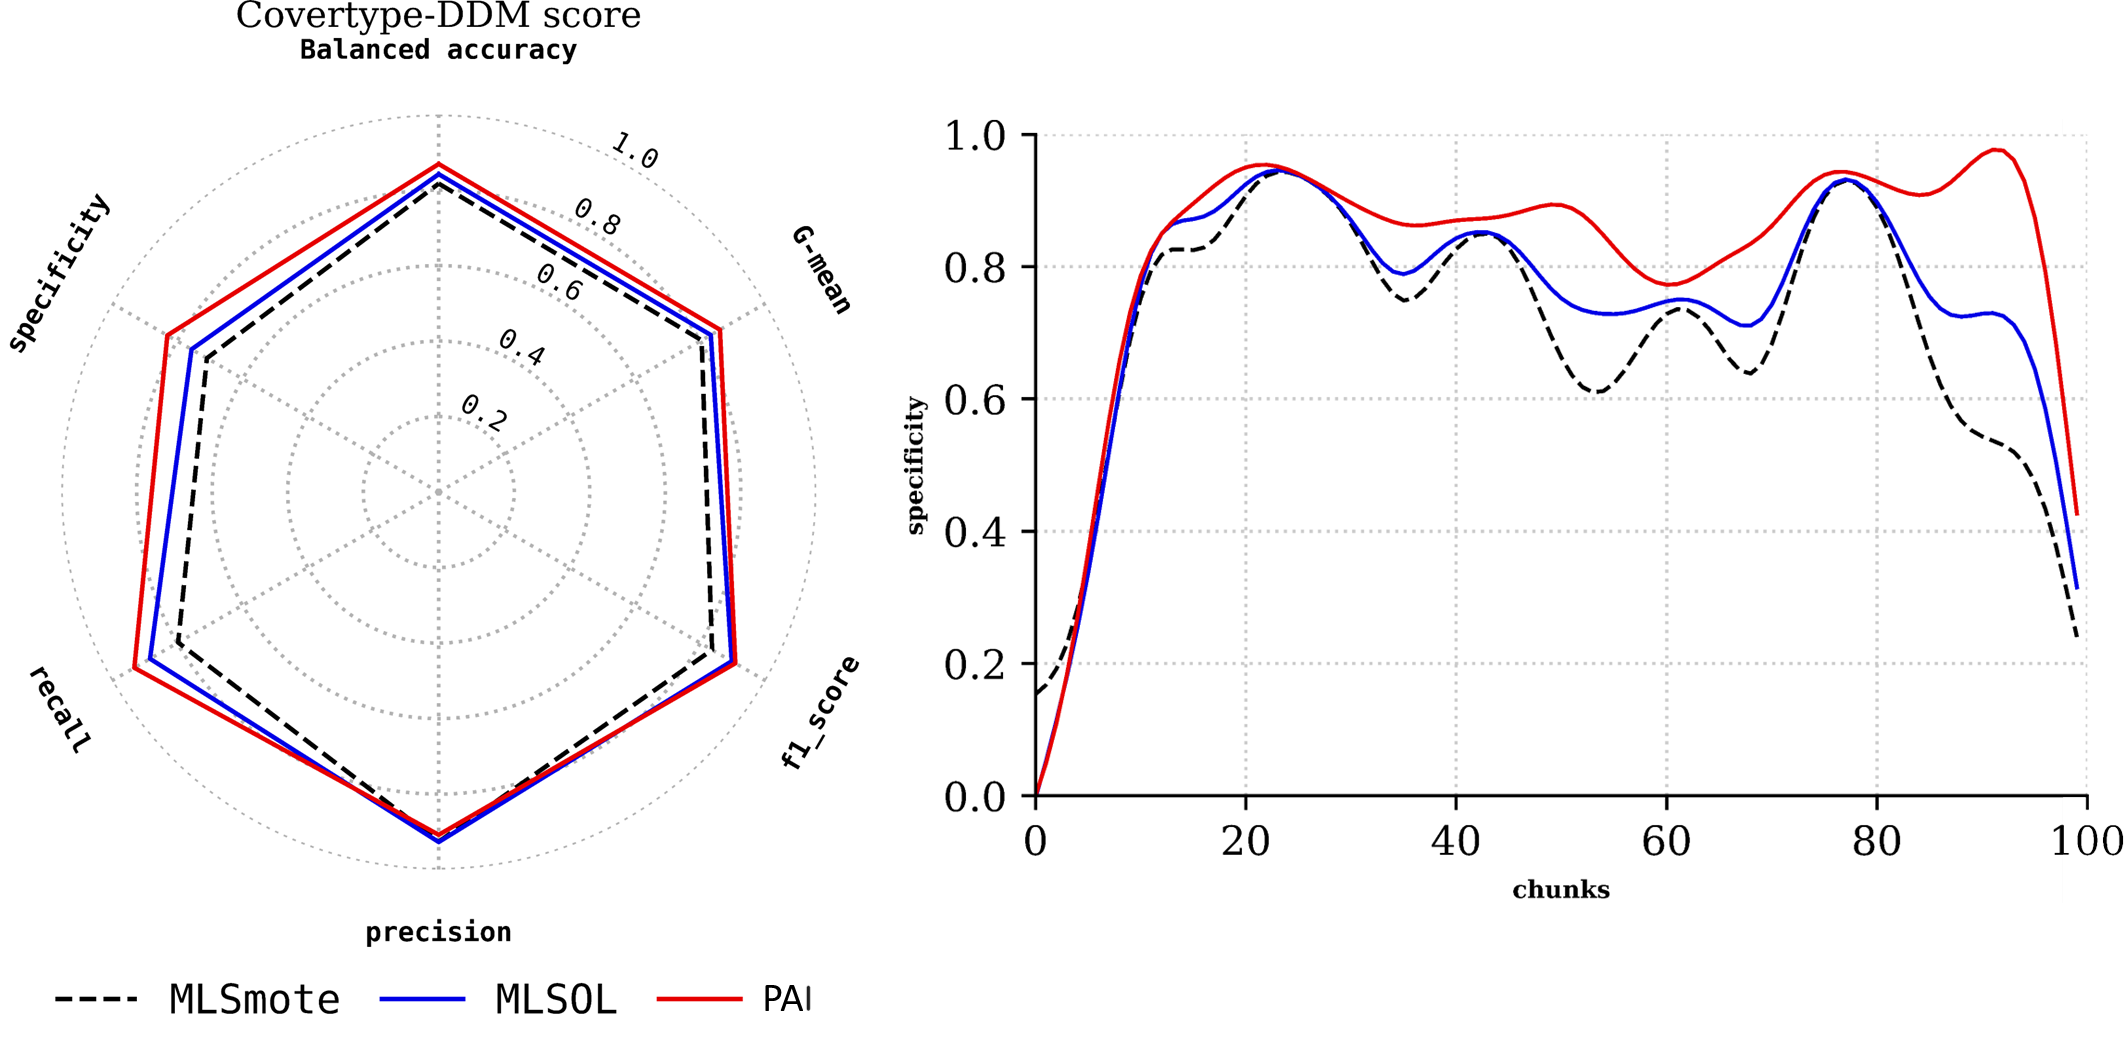
\includegraphics[width=1\linewidth]{4_Imbalanced/figures/exp_2.png}
  \caption{Comparison of PA1, MLSMOTE, and MLSOL on Covertype Dataset with DDM Concept Drift Detector.}
	\label{fig:4_first_proposal_result_exp_2}
\end{figure}

\subsubsection{Results on the Real Application Stream}
Figures \ref{fig:4_first_proposal_result_exp_3} and \ref{fig:4_first_proposal_result_exp_4} illuminate the nuanced performance dynamics of PA1, MLSMOTE, and MLSOL on the Sensor data stream, as guided by ADWIN and DDM as concept drift detectors, respectively. These visualizations encapsulate the intricate interplay between the methods and the ever-changing nature of the Sensor data stream, characterized by inherent drift and imbalance. In Figure \ref{fig:4_first_proposal_result_exp_3}, ADWIN, as a drift detector, provides a fertile ground for the methods to showcase their potential. The radar plot reveals that PA1 consistently outperforms MLSMOTE and MLSOL across most metrics, with a pronounced edge in specificity, $f_1$ score, balanced accuracy, and G-mean. This dominance speaks to PA1’s philosophical alignment with the complexities of evolving data streams, where achieving equilibrium between sensitivity and precision is paramount. The nearly identical precision and recall values among all methods suggest that MLSMOTE and MLSOL address the basic challenges of imbalanced streams adequately, yet they lack the strategic depth and adaptability demonstrated by PA1. The temporal line plot in Figure \ref{fig:4_first_proposal_result_exp_3} adds a temporal dimension to the analysis. It reveals PA1’s journey of adaptation, where its early struggle during the initial 30 chunks mirrors the challenge of limited classifier diversity. Beyond chunk 30, PA1’s ascent is unmistakable, achieving stability and sustained superiority in specificity as it harmonizes sensitivity and specificity. Meanwhile, MLSMOTE and MLSOL exhibit sporadic fluctuations, with neither achieving the same level of consistent adaptability, underscoring their comparative limitations.

In contrast, Figure \ref{fig:4_first_proposal_result_exp_4} shifts the lens to DDM as the drift detector. The radar plot reveals a general decline in metric values compared to ADWIN, reflecting DDM’s limitations in capturing subtle drift nuances. However, the line plot continues to affirm PA1’s resilience and dominance. Despite the overall convergence of performance among the three methods over time, PA1 remains the most stable and adaptable, consistently achieving higher specificity values even under the more rigid framework imposed by DDM. This performance gap highlights the sensitivity of drift detection mechanisms to the data stream's characteristics and emphasizes the importance of matching drift detection strategies with the demands of the learning algorithm.

The juxtaposition of Figures \ref{fig:4_first_proposal_result_exp_3} and \ref{fig:4_first_proposal_result_exp_4} serves as a philosophical reflection on the intricate interdependencies between drift detection and classifier performance. ADWIN emerges as a more capable arbiter of change, enabling PA1 to leverage its full potential. In contrast, DDM’s rigidity underscores the challenges of achieving optimal adaptability in dynamic environments. Yet, PA1’s persistent robustness across both scenarios affirms its role as a paradigm of adaptability and resilience. These findings underscore the importance of harmonizing classifier ensemble design with drift detection mechanisms to navigate the multifaceted challenges posed by real-world, non-stationary, and imbalanced data streams. PA1’s ability to sustain high performance across metrics and adapt to diverse drift conditions exemplifies the convergence of algorithmic innovation and the philosophical pursuit of balance in machine learning. In this context, specificity emerges as a profound metric, embodying the trade-offs and synergies required to achieve holistic success in evolving data environments.
 
\begin{figure}[H]
	\centering
	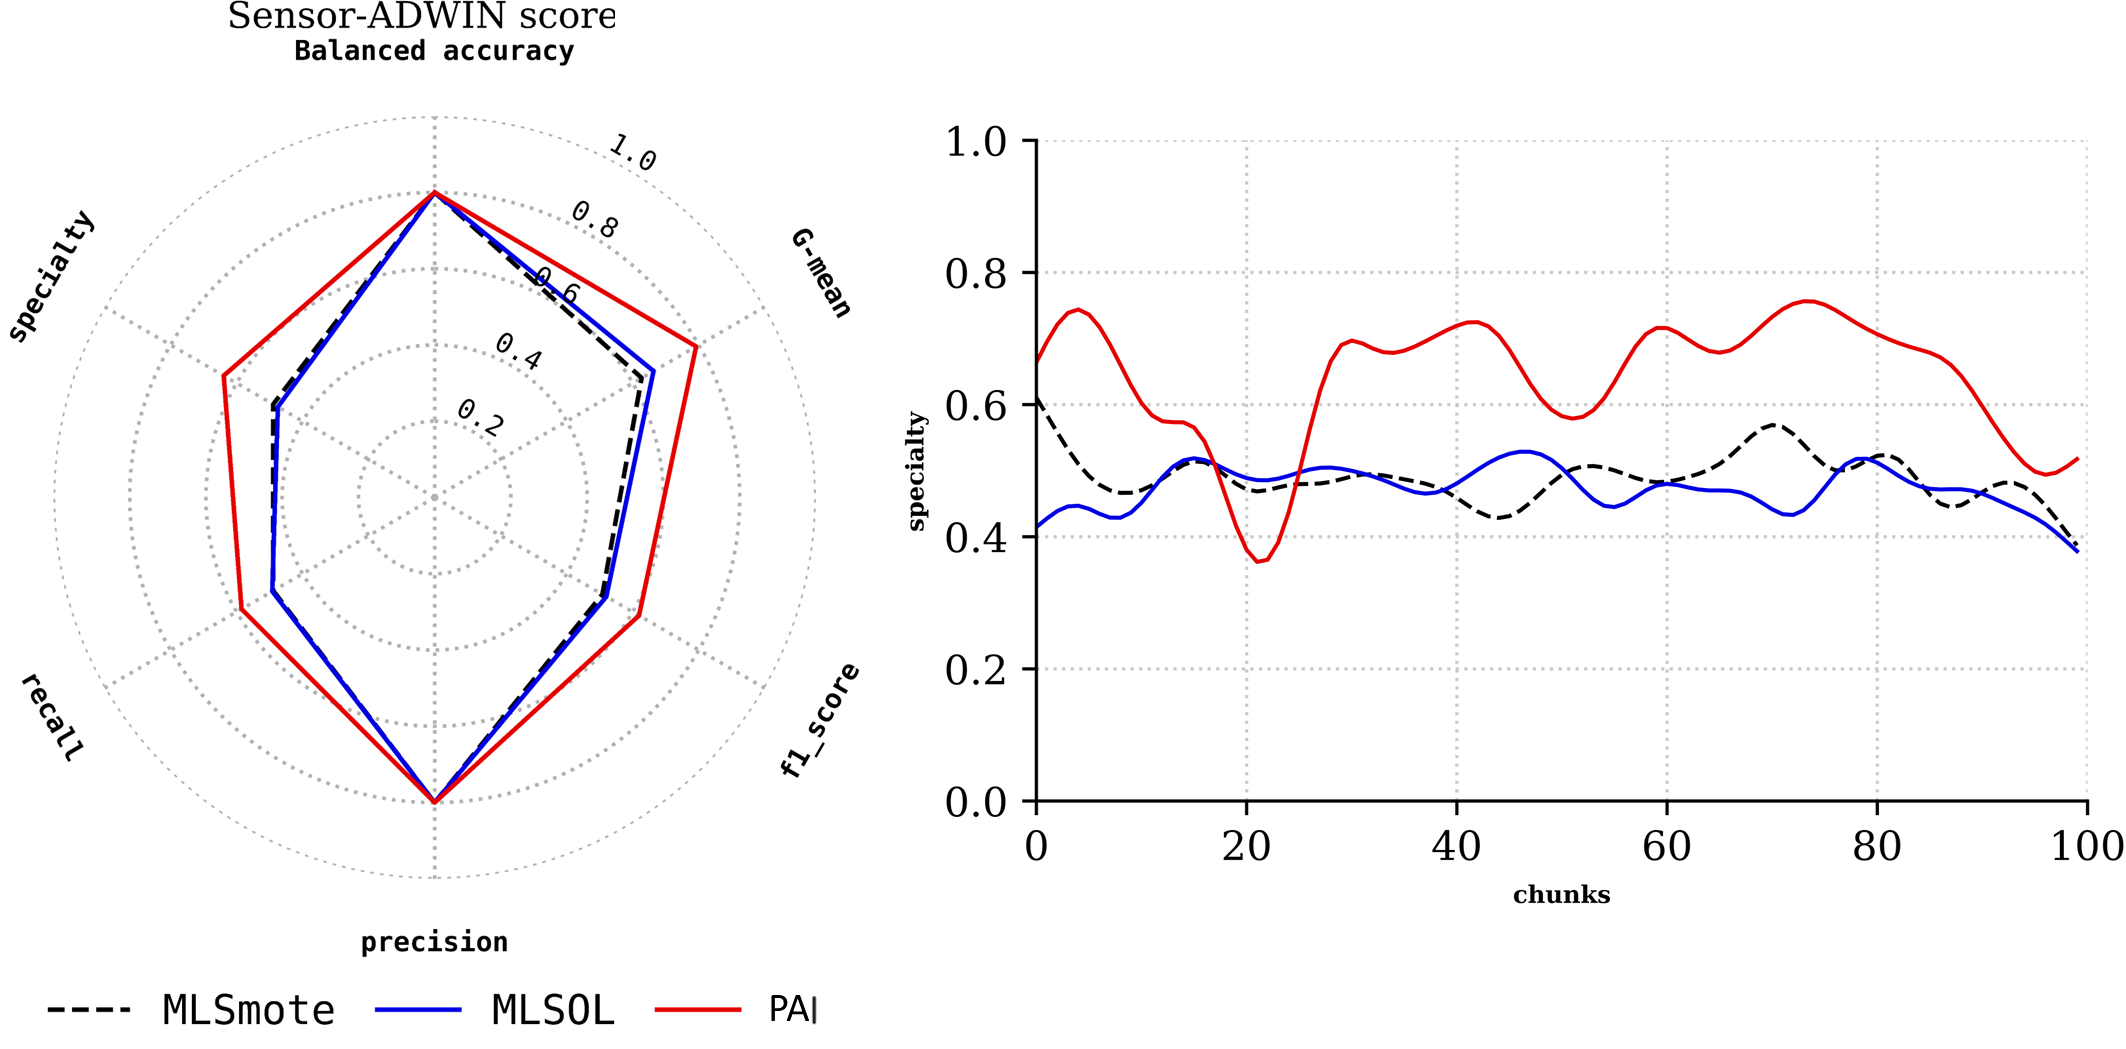
\includegraphics[width=1\linewidth]{4_Imbalanced/figures/exp_3.png}
  \caption{Comparison of PA1, MLSMOTE, and MLSOL on Sensor Dataset with ADWIN Concept Drift Detector.}
	\label{fig:4_first_proposal_result_exp_3}
\end{figure}

\begin{figure}[H]
	\centering
	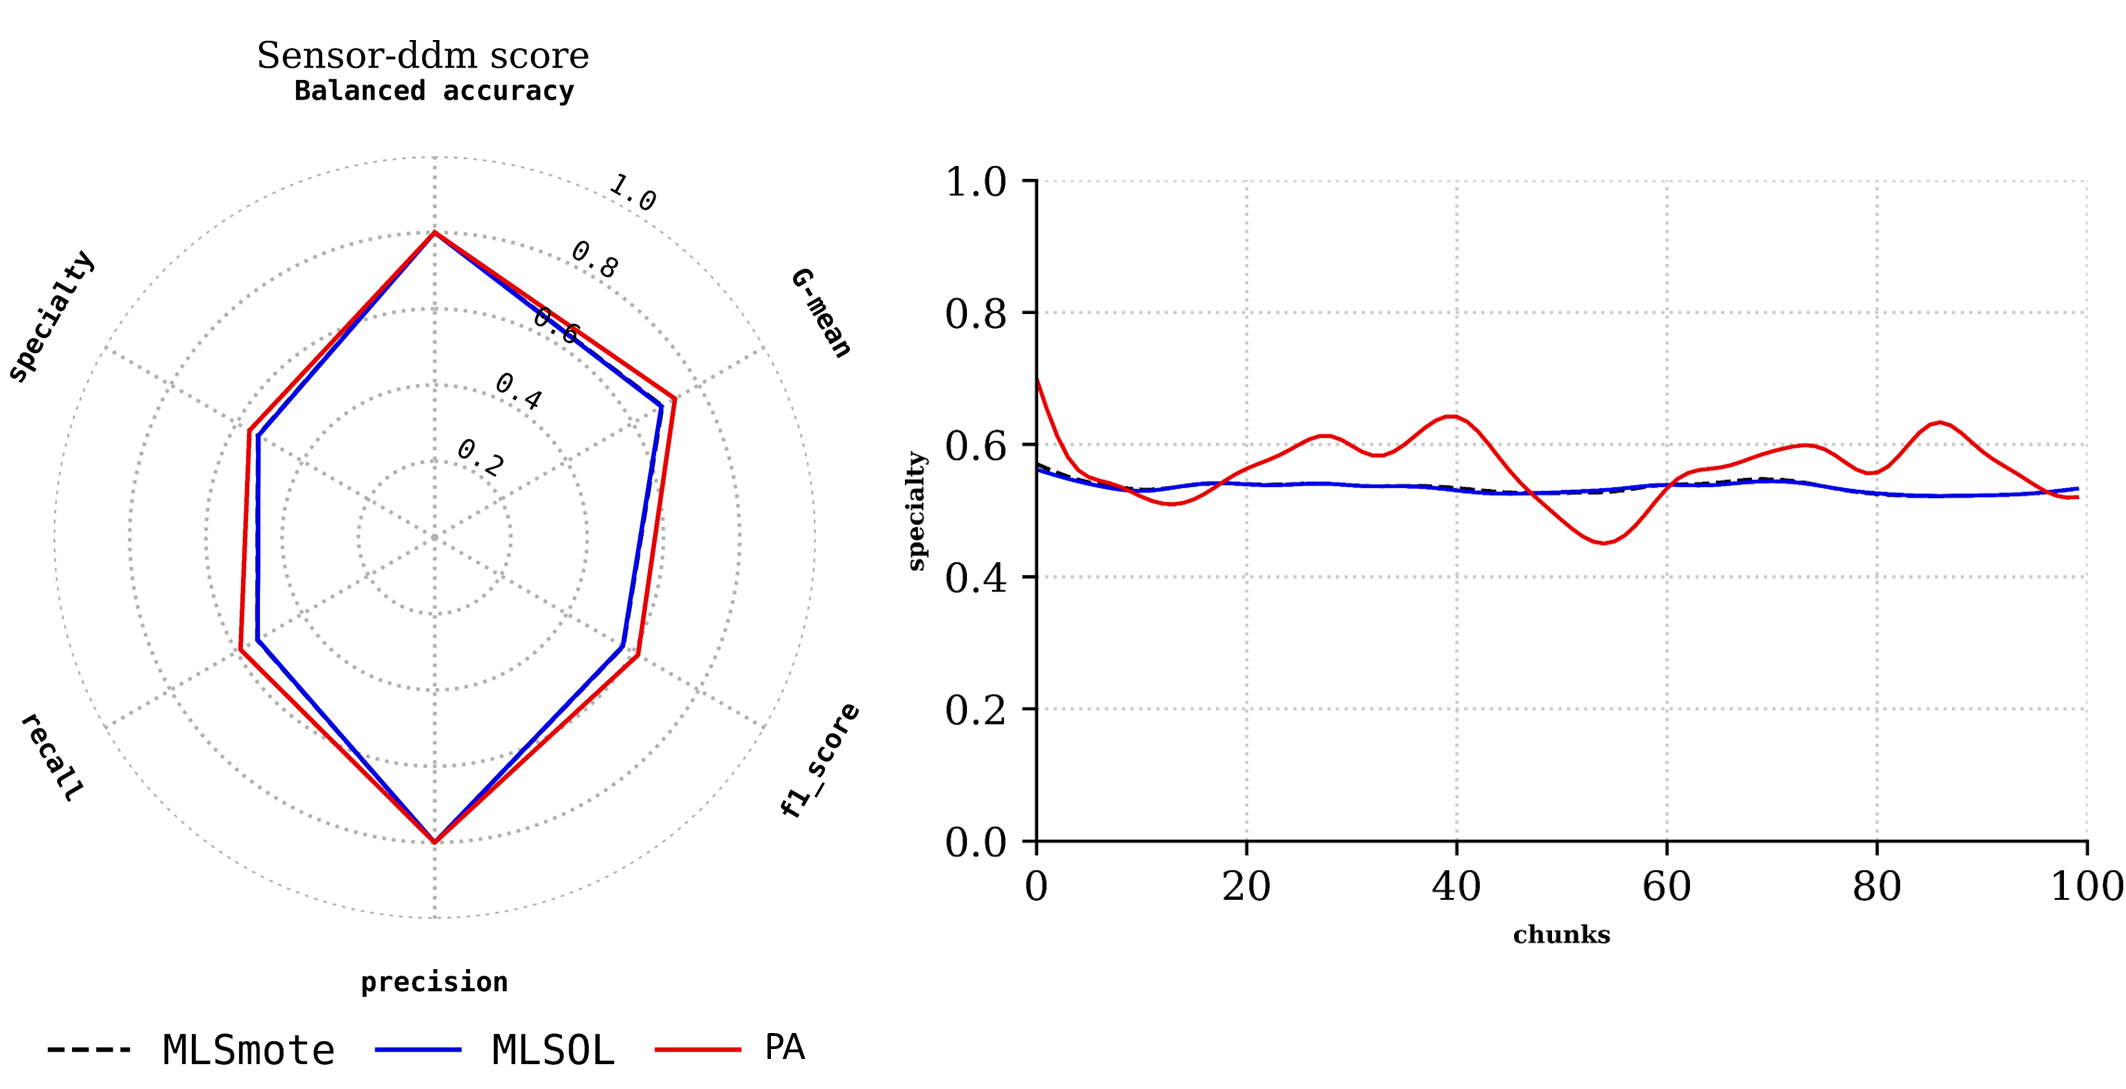
\includegraphics[width=1\linewidth]{4_Imbalanced/figures/exp_4.png}
  \caption{Comparison of PA1, MLSMOTE, and MLSOL on Sensor Dataset with DDM Concept Drift Detector}.
	\label{fig:4_first_proposal_result_exp_4}
\end{figure}

\subsubsection{Results on the Synthetic Stream}
Figures \ref{fig:4_first_proposal_result_exp_5} and \ref{fig:4_first_proposal_result_exp_6} delve into the interplay of algorithms and concept drift detectors on synthetic data streams, offering a profound narrative on adaptability and resilience amidst frequent and abrupt changes. In Figure \ref{fig:4_first_proposal_result_exp_5}, ADWIN acts as the sentinel of change, facilitating an environment that reveals the nuanced strengths and limitations of each method. The radar plot paints a vivid portrait of metric values clustering between 0.6 and 0.8, symbolizing the relentless nature of synthetic data drifts. Within this chaotic landscape, MLSOL stands out with its precision, an achievement that reflects its singular focus on minimizing false positives. However, this narrow emphasis leaves it vulnerable across other metrics. Conversely, MLSMOTE's consistent underperformance highlights its inability to navigate the complexities of frequent drifts effectively. PA1, in contrast, emerges as a paradigm of balance and adaptability. Its superiority across metrics other than precision is not merely a testament to its robustness but also a reflection of its philosophical alignment with the dynamic nature of non-stationary streams. The transitional phase observed during the first ten chunks, where PA1 struggles, mirrors the natural process of adaptation: a period of recalibration before achieving mastery. Once this initial inertia is overcome, PA1 demonstrates a sustained trajectory of excellence, harmonizing the competing demands of sensitivity and specificity. The line plot becomes a visual metaphor for resilience—PA1 not only adapts to but thrives within the evolving challenges of the data stream.

Figure \ref{fig:4_first_proposal_result_exp_6} extends this narrative under the gaze of DDM, a drift detector with a contrasting philosophy to ADWIN. While the radar plot reaffirms the earlier insights, it is the subtle degradation in MLSOL and MLSMOTE’s performance that becomes a focal point. This decline underscores their dependence on the nuances of the drift detection mechanism, revealing their fragility when faced with an altered evaluative lens. PA1, however, remains steadfast, its consistent superiority reaffirming its ability to transcend the limitations of individual drift detectors. This resilience highlights the algorithm's intrinsic capacity for adaptability, a hallmark of effective learning in uncertain environments. The comparative analysis between ADWIN and DDM unveils a deeper truth: ADWIN’s finesse in capturing abrupt and frequent drifts makes it a superior ally in handling synthetic data streams. Yet, the overarching narrative is not about the drift detectors alone but about PA1’s versatility and robustness across diverse conditions. Its ability to navigate the complexities of synthetic, Covertype, and Sensor datasets while maintaining high performance reflects a profound balance between precision and recall. PA1 embodies the ideal of equilibrium, where adaptability and robustness converge to address the multifaceted challenges of real-world, non-stationary data. Through this lens, PA1 transcends its technical role, becoming a philosophical exemplar of learning in the face of change. It illustrates that success in dynamic environments is not solely about excelling in isolated metrics but about harmonizing competing objectives to achieve sustained performance. This balance resonates with the broader challenge of adapting to non-stationarity, offering a roadmap for tackling the inherent uncertainties of real-world applications. PA1, therefore, stands not just as an effective algorithm but as a testament to the principles of adaptability, resilience, and balance that define progress in complex systems.

\begin{figure}[H]
	\centering
	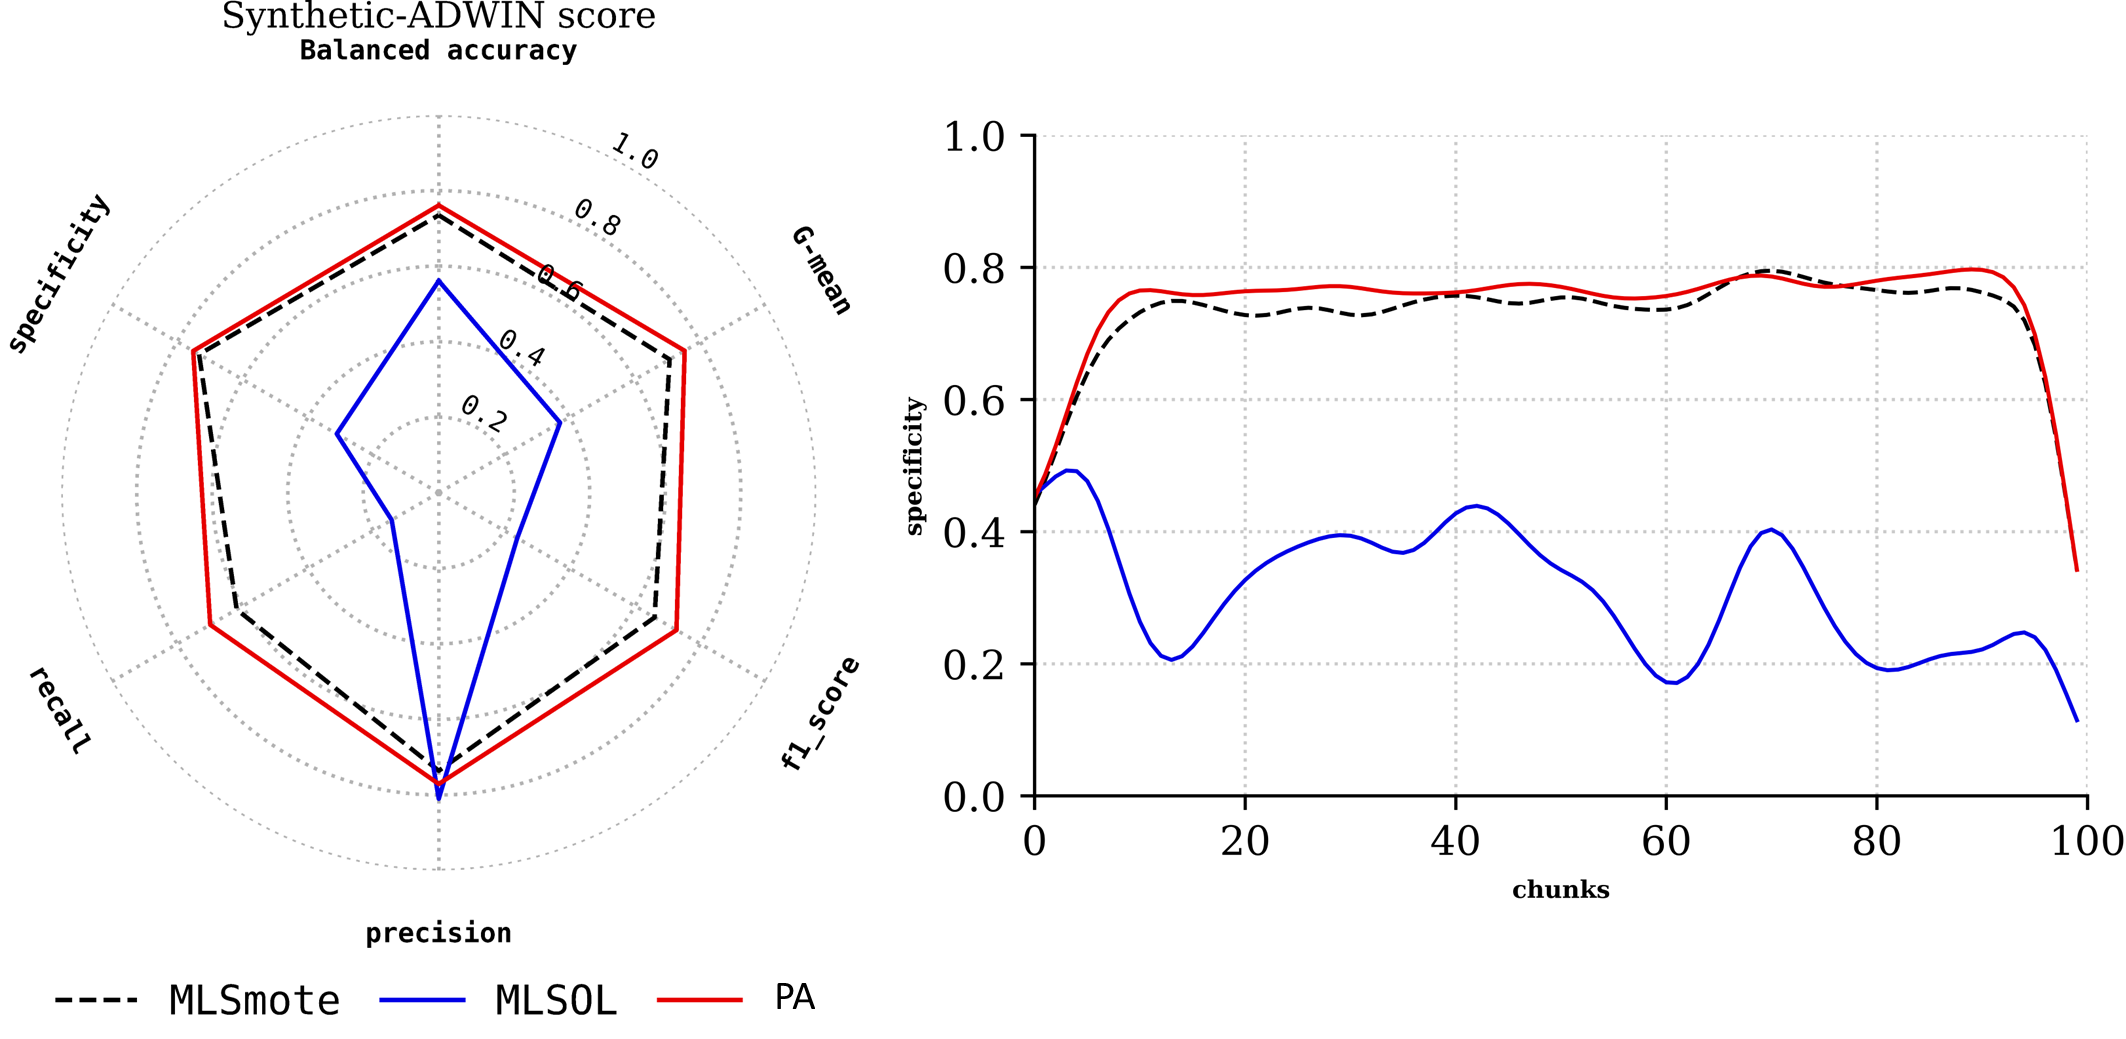
\includegraphics[width=0.8\linewidth]{4_Imbalanced/figures/exp_5.png}
  \caption{Comparison of PA1, MLSMOTE, and MLSOL on Synthetic Stream with ADWIN.}
	\label{fig:4_first_proposal_result_exp_5}
\end{figure}

\begin{figure}[H]
	\centering
	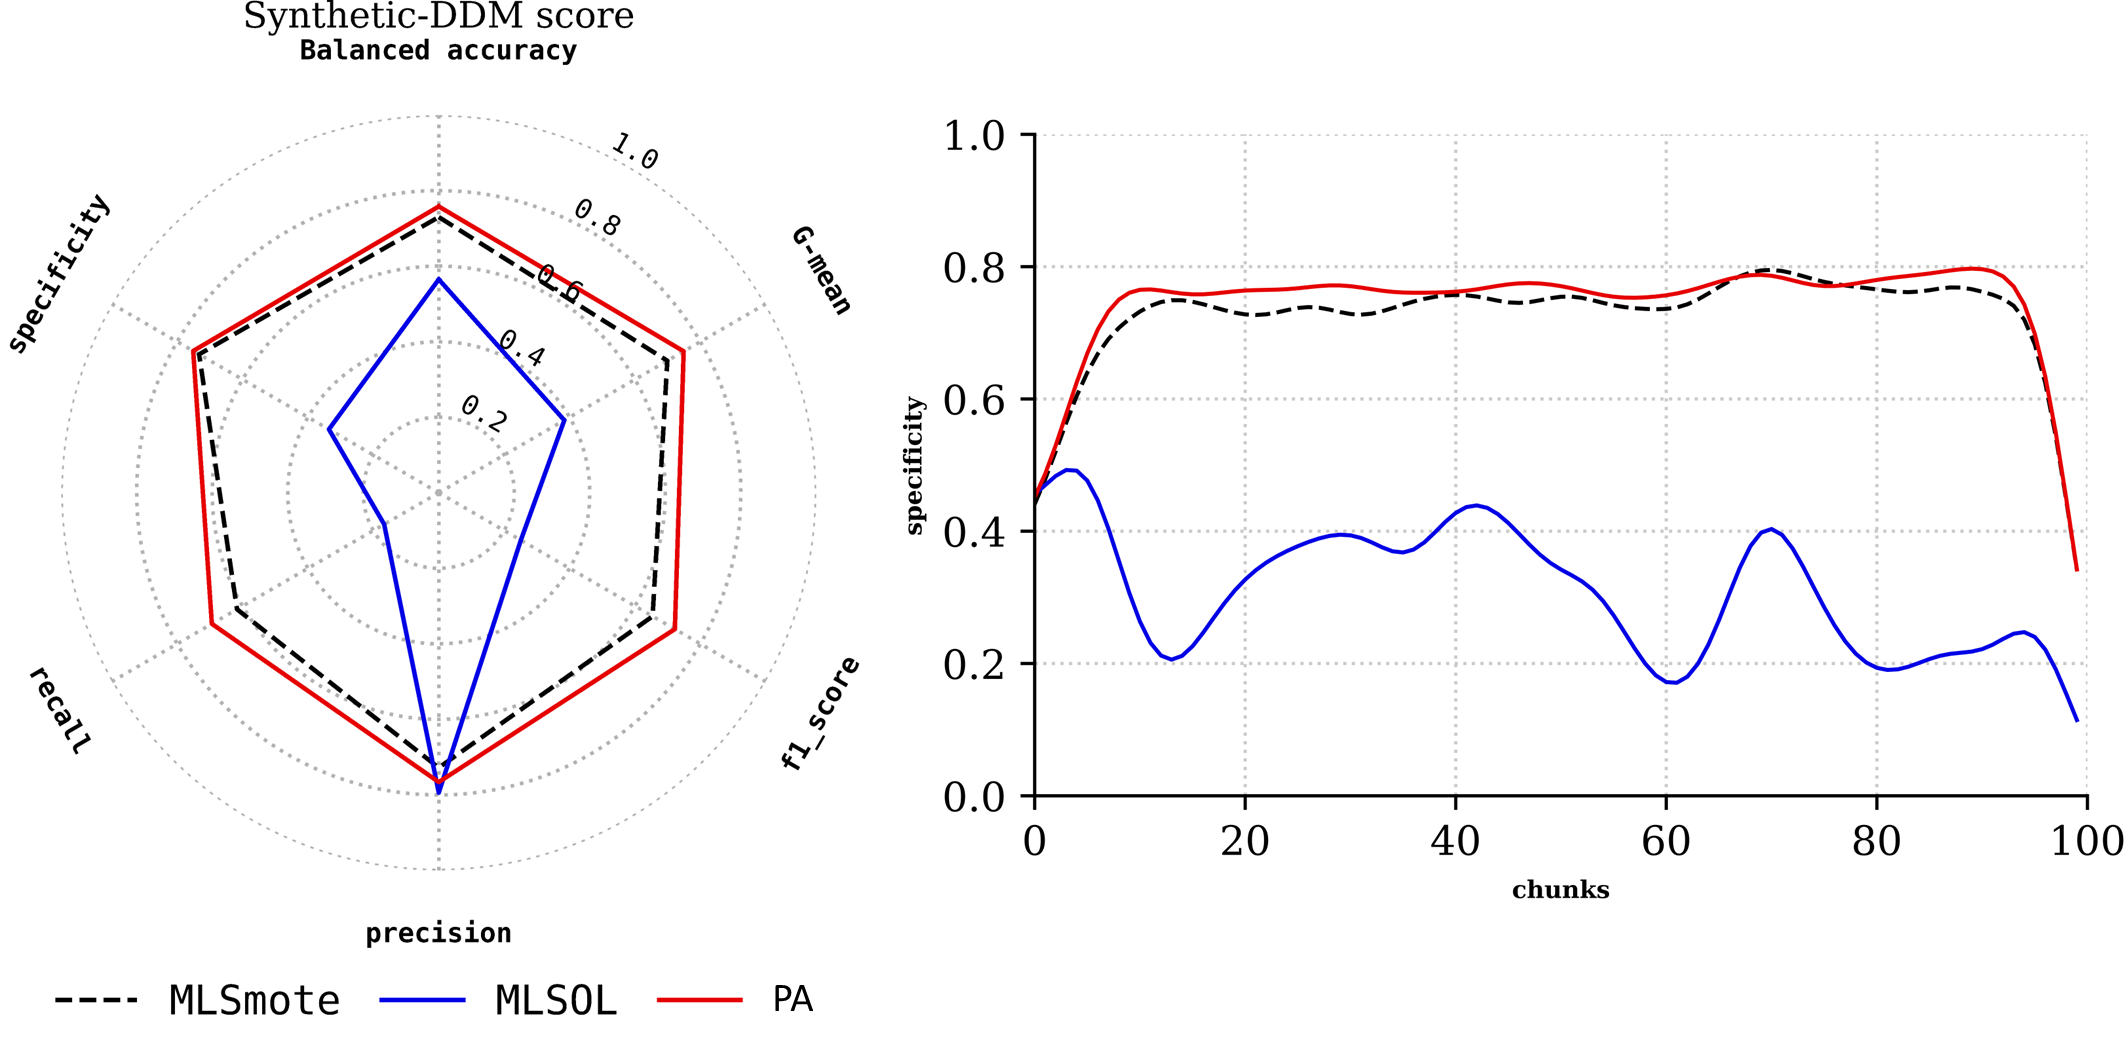
\includegraphics[width=0.8\linewidth]{4_Imbalanced/figures/exp_6.png}
  \caption{Comparison of PA1, MLSMOTE, and MLSOL on Synthetic with DDM.}
	\label{fig:4_first_proposal_result_exp_6}
\end{figure}


\subsection{Analysis of Overlapoing between PA1, MLSMOTE, and MLSOL.}
This experimental study focuses on identifying the key factors influencing the selection of optimal approaches for addressing minority class challenges in imbalanced and drifted data streams. The factors under consideration include dataset characteristics, the choice of concept drift detection methods, and the algorithm's capability to minimize class overlap.
The concept of overlapping classes refers to situations where instances from different classes in a dataset share similar feature values, making it difficult to distinguish between them. This overlap complicates classification tasks, as the boundaries between classes become less distinct. To evaluate these aspects, the overlapping class behavior of the first proposed approach (PA1) was compared with MLSMOTE and MLSOL through experiments grouped into ten chunks each. Results were visualized using bar diagrams, where each bar represents the number of overlapping samples for ten chunks of various data streams under two drift detectors, ADWIN and DDM. Figures \ref{fig:4_first_proposal_result_exp_7}, \ref{fig:4_first_proposal_result_exp_8}, and \ref{fig:4_first_proposal_result_exp_9} present the experimental outcomes. Each figure contains ten bar groups, where each group represents overlapping samples for chunks processed by MLSMOTE, MLSOL, and PA1.
\begin{figure}[H]
	\centering
	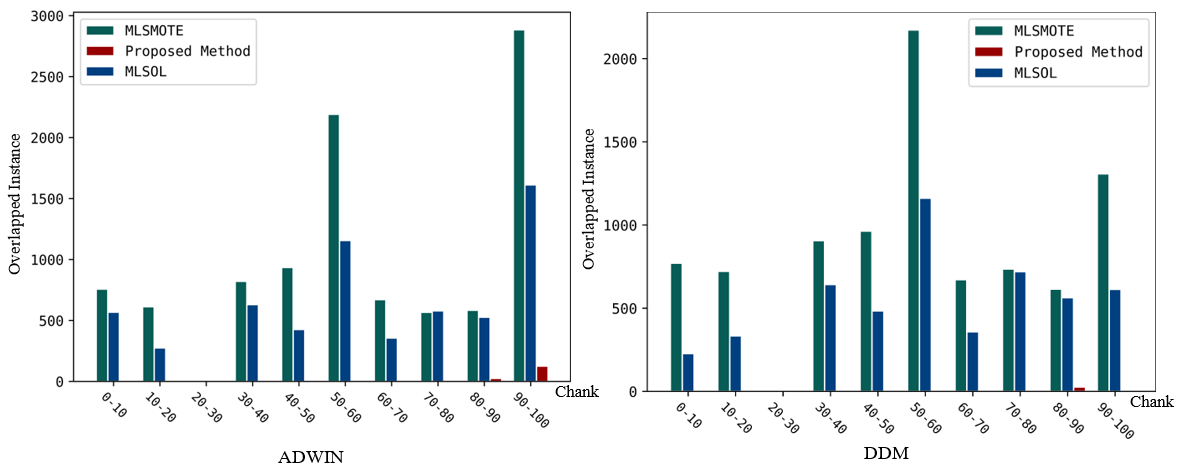
\includegraphics[width=0.9\linewidth]{4_Imbalanced/figures/exp_7.png}
  \caption{Overlapping Points of PA1, MLSMOTE, and MLSOL on Covertype Stream.}
	\label{fig:4_first_proposal_result_exp_7}
\end{figure}
Figure \ref{fig:4_first_proposal_result_exp_7}:
This figure highlights overlapping samples for a synthetic stream under both ADWIN and DDM drift detectors. The ADWIN diagram shows reduced overlapping samples for chunks 20–30 due to the absence of concept drifts, which eliminated the generation of synthetic samples. Conversely, chunks 60–70 and 90–100 exhibit the highest number of overlapping samples, corresponding to frequent drifts. Across all chunk groups, MLSMOTE generates the most overlapping samples, while PA1 consistently records the lowest overlap, except in the final group (chunks 90–100). In comparison, the DDM diagram exhibits more overlapping samples than the ADWIN diagram because DDM detects fewer drifts, resulting in prolonged training on outdated models. The highest Y-axis value in the ADWIN diagram reaches 3,000 samples, while in the DDM diagram, it is 2,000 samples, emphasizing the difference in drift sensitivity between the detectors. Figure \ref{fig:4_first_proposal_result_exp_8}:
This figure compares the overlapping sample behavior of the three methods on the Sensor stream. The ADWIN diagram demonstrates fewer overlapping samples than in Figure \ref{fig:4_first_proposal_result_exp_7}, indicating a lower number of drifts in the Sensor dataset. The results further confirm PA1’s effectiveness in minimizing overlapping samples compared to MLSOL and MLSMOTE, with MLSMOTE consistently exhibiting the highest overlap. For the DDM diagram, the number of overlapping samples is lower than in the ADWIN diagram, reinforcing PA1’s advantage in reducing overlap, even under fewer detected drifts.
\begin{figure}[H]
	\centering
	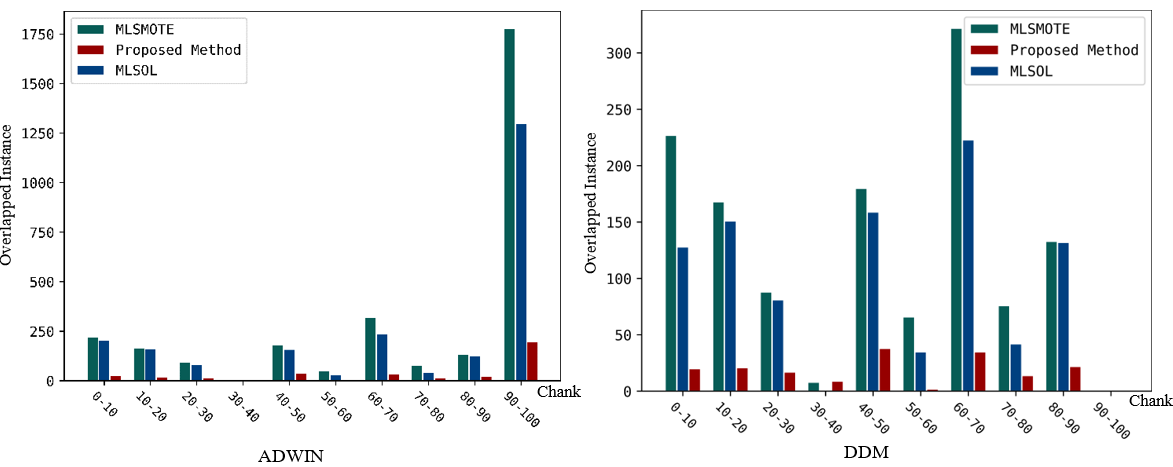
\includegraphics[width=0.9\linewidth]{4_Imbalanced/figures/exp_8.png}
  \caption{Overlapping Points of PA1, MLSMOTE, and MLSOL on Sensor Stream.}
	\label{fig:4_first_proposal_result_exp_8}
\end{figure}
Figure \ref{fig:4_first_proposal_result_exp_9}:
This figure examines overlapping samples in the synthetic data stream, where the ADWIN and DDM diagrams exhibit the largest number of overlapping samples compared to earlier figures. This indicates that the synthetic stream experienced frequent drifts and greater noise levels. The highest Y-axis value for both diagrams reaches 7,000 samples. Despite this, PA1 maintains the lowest overlapping sample count across most groups, while MLSMOTE records the highest overlap consistently, regardless of the drift detector employed.
\begin{figure}[H]
	\centering
	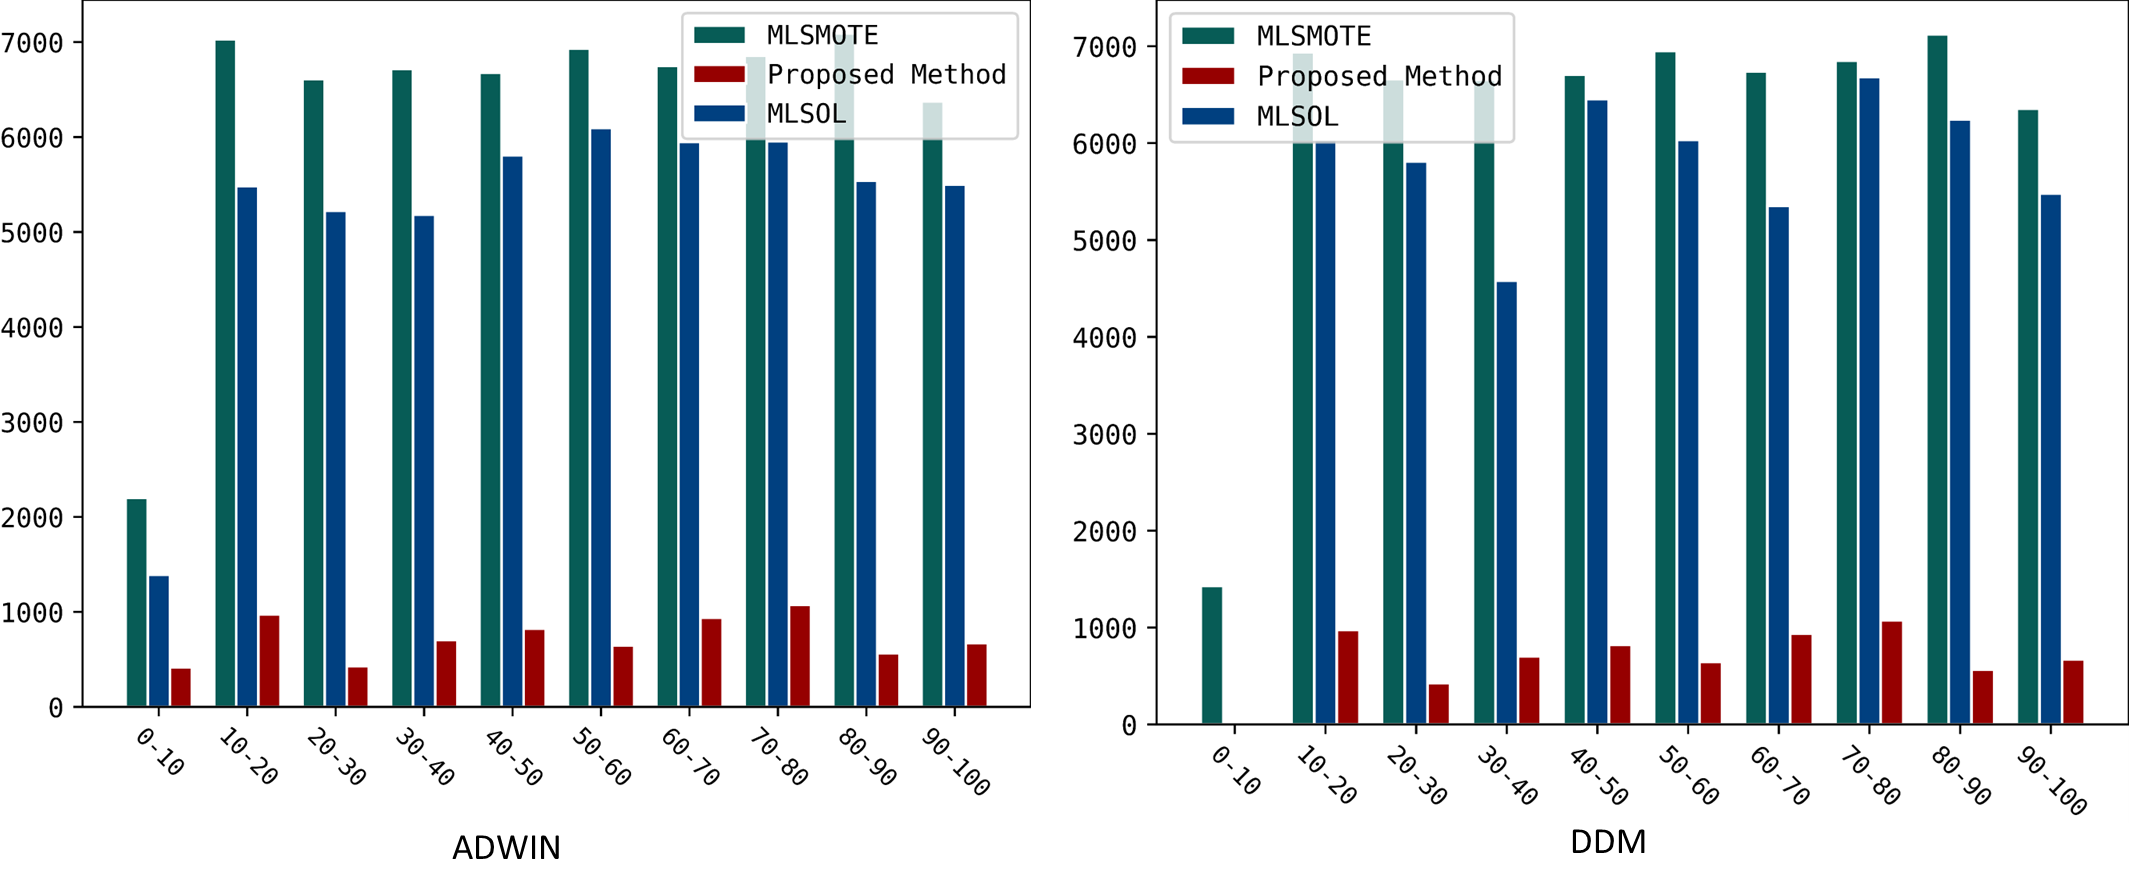
\includegraphics[width=0.9\linewidth]{4_Imbalanced/figures/exp_9.png}
  \caption{Overlapping Points of PA1, MLSMOTE, and MLSOL on Synthetic Stream.}
	\label{fig:4_first_proposal_result_exp_9}
\end{figure}

\subsection{Analyzing Runtime Between PA1, MLSMOTE, and MLSOL.}

The runtime of an algorithm encapsulates its operational efficiency, representing the total time consumed during both training and prediction phases over a data stream. Measured in seconds, runtime serves as a critical metric that reflects not just computational performance but also the algorithm's ability to adapt to dynamic challenges like concept drift while delivering predictions.

In Table \ref{tab:4_first_proposal_result_table_2}, runtime metrics are compared across the proposed approach and other methods, including MLSMOTE and MLSOL, applied to datasets such as Covertype, Sensor, and synthetic data streams. The recorded runtimes provide a clear narrative of computational efficiency. For instance, using the ADWIN concept drift detector, the proposed approach required 8344 seconds to process the Covertype dataset with ensemble classifiers. A slight reduction in runtime was observed when DDM was employed, with the runtime decreasing to 8019 seconds. These observations highlight the algorithm’s adaptability and its ability to optimize performance under varying drift detection mechanisms. Comparatively, the proposed approach demonstrates a consistently shorter runtime than MLSMOTE and MLSOL across all datasets and drift detectors. This superiority is emphasized in the table through bolded runtime values, underscoring the efficiency advantage of the proposed algorithm. Such efficiency stems from its innovative ability to reduce the generation of overlapping samples during training, effectively minimizing redundant computational overhead. This design not only streamlines training processes but also accelerates prediction phases, a critical requirement for real-time data streams. The choice of drift detector further influences runtime dynamics. DDM, characterized by a lower rate of drift detection compared to ADWIN, leads to fewer instances where classifier retraining is triggered. This reduction in training frequency directly contributes to the observed decrease in runtime when DDM is used. However, the slightly higher runtime with ADWIN reflects its sensitivity to detecting more frequent and abrupt concept drifts, which necessitates more frequent retraining of classifiers. While this increases computational demands, it also ensures robust adaptation to rapidly changing data streams.

By reducing computational effort through fewer overlapped samples and aligning seamlessly with drift detection mechanisms, the proposed algorithm establishes itself as a practical solution for handling non-stationary data. This efficiency is particularly vital in real-world applications, where processing speed and responsiveness are as critical as predictive accuracy. The findings emphasize the importance of algorithmic design choices in optimizing runtime, reaffirming the proposed approach’s position as a robust, scalable, and efficient solution for real-time data stream processing.

\begin{table}[H]
  \centering
  \caption{Runtimes (in seconds) Comparison of PA1, MLSMOTE, and MLSOL.}
  \resizebox{\textwidth}{!}{
  \begin{tabular}{|l|l|c|c|c|}
  \hline
  \textbf{Stream} & \textbf{Concept Drift Detector} & \textbf{MLSMSOTE} & \textbf{MLSOL} & \textbf{PA1} \\ \hline
  \multirow{2}{*}{Benchmark} & ADWIN & 9559 & 8655 & \textbf{8344} \\ \cline{2-5} 
   & DDM & 8388 & 8031 & \textbf{8019} \\ \hline
  \multirow{2}{*}{Real Application} & ADWIN & 1291 & 1310 & \textbf{1102} \\ \cline{2-5} 
   & DDM & 585 & 607 & \textbf{521} \\ \hline
  \multirow{2}{*}{Synthetic} & ADWIN & 12870 & 4866 & \textbf{4834} \\ \cline{2-5} 
   & DDM & 12397 & 4958 & \textbf{4687} \\ \hline
  \end{tabular}
  }
  \label{tab:4_first_proposal_result_table_2}
  \end{table}

\subsection{Analyzing Non-parametric Tests between PA1, MLSMOTE, and MLSOL.}
A comprehensive statistical analysis was performed, encompassing 12 experimental comparisons across three distinct datasets, three algorithms (PA1, MLSMOTE, and MLSOL), and two concept drift detection mechanisms (ADWIN and DDM). To ensure rigor, the Kruskal-Wallis test, a non-parametric statistical method, was employed to evaluate the differences in G-mean performance across the experiments. The results of the Kruskal-Wallis test revealed substantial variations in G-mean values, underscoring the influence of the algorithms and drift detectors on performance outcomes. These observed differences were statistically significant and unlikely to result from random chance \cite{yamada2013change}. This conclusion was drawn based on the acceptance or rejection of the null hypothesis (H0), which posits that no significant differences exist between the groups. The null hypothesis was accepted in most experiments, indicating statistically significant disparities between expected and observed data. Acceptance of H0 was contingent upon the P-value falling below a critical threshold, which was determined at a 95\% confidence level.
\begin{table}[H]
  \centering
  \caption{Kruskal-Wallis test results for MLSMOTE, MLSOL, and PA1.}
  \resizebox{\textwidth}{!}{
  \begin{tabular}{|c|c|c|c|c|c|}
  \hline
  \multirow{2}{*}{Dataset} & \multirow{2}{*}{Drift detector} & \multirow{2}{*}{Comparison} & \multirow{2}{*}{P-value} & \multirow{2}{*}{Critical value} & \multirow{2}{*}{H0} \\ 
                           &                                 &                             &                           &                                 &  \\
  \hline
  \multirow{4}{*}{Covertype stream} & \multirow{2}{*}{ADWIN} & PA1 - MLSSMOTE & 0.001 & 0.05 & Accept \\ \cline{3-6}
                                    &                        & PA1 - MLSOL    & 0.014 & 0.05 & Accept \\ \cline{2-6}
                                    & \multirow{2}{*}{DDM}   & PA1 - MLSSMOTE & 0.361 & 0.05 & Rejected \\ \cline{3-6}
                                    &                        & PA1 - MLSOL    & 0.401 & 0.05 & Rejected \\ 
  \hline
  \multirow{4}{*}{Sensor stream} & \multirow{2}{*}{ADWIN} & PA1 - MLSSMOTE & 0.001 & 0.05 & Accept \\ \cline{3-6}
                                 &                        & PA1 - MLSOL    & 0.001 & 0.05 & Accept \\ \cline{2-6}
                                 & \multirow{2}{*}{DDM}   & PA1 - MLSSMOTE & 0.001 & 0.05 & Accept \\ \cline{3-6}
                                 &                        & PA1 - MLSOL    & 0.001 & 0.05 & Accept \\ 
  \hline
  \multirow{4}{*}{Synthetic stream} & \multirow{2}{*}{ADWIN} & PA1 - MLSSMOTE & 0.001 & 0.05 & Accept \\ \cline{3-6}
                                    &                        & PA1 - MLSOL    & 0.001 & 0.05 & Accept \\ \cline{2-6}
                                    & \multirow{2}{*}{DDM}   & PA1 - MLSSMOTE & 0.001 & 0.05 & Accept \\ \cline{3-6}
                                    &                        & PA1 - MLSOL    & 0.001 & 0.05 & Accept \\ 
  \hline
  \end{tabular}
  }
  \label{tab:4_first_proposal_result_table_3}
  \end{table}
For precision and clarity, the P-value was rounded to three decimal places.
Table \ref{tab:4_first_proposal_result_table_3} provides detailed insights into the comparative performances of the three methods. The statistical results consistently highlighted the superiority of PA1 in handling non-stationary and imbalanced data streams, supported by significant variations in G-mean across most experiments. However, in the third and fourth experiments, a notable similarity in the performance of PA1, MLSMOTE, and MLSOL emerged, leading to the rejection of H0. This convergence in performance can be attributed to the behavior of the DDM drift detector, which identified fewer concept drifts in these particular experiments. The reduced drift detection frequency by DDM likely diminished the opportunities for the algorithms to exhibit their adaptive capabilities, resulting in a more uniform performance across methods. This statistical analysis underscores the nuanced interplay between drift detection mechanisms and algorithmic performance. The ADWIN detector, with its heightened sensitivity to frequent drifts, consistently highlighted performance differences among the methods, enabling a clearer evaluation of their capabilities. In contrast, the less sensitive DDM detector contributed to the observed convergence in performance, emphasizing the impact of drift detection frequency on experimental outcomes. The significant disparities observed in most experiments validate the robustness of PA1 and highlight the necessity of harmonizing algorithmic design with appropriate drift detection mechanisms to address the challenges of non-stationary and imbalanced datasets effectively.
